\documentclass[letterpaper,12pt]{article}
\usepackage{graphicx,amsmath} % support the \includegraphics command and options
\usepackage{color}
\usepackage{hyperref,float}
\usepackage{dgjournal} 
%\usepackage{mathptmx}
\usepackage[authoryear,comma,longnamesfirst,sectionbib]{natbib} 

\newcommand{\andyc}[1]{[{\color{red}\sc Andy says: {\tt #1}}]}
\newcommand{\scotlandc}[1]{[{\color{red}\sc Scotland says: {\tt #1}}]}
\newcommand{\lucasc}[1]{[{\color[rgb]{0,0.7,0}\sc Lucas says: {\tt #1}}]}
\newcommand{\xinranc}[1]{[{\color{red}\sc Xinran says: {\tt #1}}]}
\newcommand{\yuhyunc}[1]{[{\color{red}\sc Yuhyun says: {\tt #1}}]}
\newcommand{\ianc}[1]{[{\color{red}\sc Ian says: {\tt #1}}]}
\newcommand{\marcosc}[1]{[{\color{blue}\sc Marcos is confused and says: {\tt #1}}]}

\oddsidemargin=0.25in
\evensidemargin=0.25in
\textwidth=6in
\textheight=8.75in
\topmargin=-.5in
\footskip=0.5in

\graphicspath{{figures/}{../figures/}}

\title{Nearest-Neighbor Matchup Effects:  Accounting for team match ups in the NCAA tournament}
 \author{The Lemanski Sports Analytics Group}        
\begin{document}
%% Do NOT include any fronmatter information; including the title, author names,
%% institutes, acknowledgments and title footnotes (author information, funding
%% sources, etc.). Start the document with the first section or paragraph of
%% the article.


\originalmaketitle
\section*{Task Summary:  Final Manuscript Due July 15}

\subsubsection*{Writing Assignments:}
\begin{itemize}
\item Andy: Data, Modeling, Evaluation, Recommendations, Discussion
\item Ian: Introduction, including Lit Review
\item Lucas: Luck
\item Marcos: Recommendations, Decision Theory
\item Scotland: all
\item Xinran: Evaluation, maybe modeling
\item Yuhyun: Introduction, including Lit Review
\end{itemize}
%%%%%%%%%%%%%%%%%%%%%%%%%%%%%%%%%%%%%%%%%%%
\section{Introduction}
Every March, millions of people take to an American tradition, filling out an NCAA tournament bracket. There are numerous ways to fill out a bracket. Typical strategies include using the tournament seeds, listening to so-called experts on tv or the Internet, or following one's intuition. The rise in sports analytics and the popularity of sites such as Nate Silver's fivethirtyeight.com is increasing the visibility of data-driven methods for NCAA tournament predictions. Predictive tournament challenges, such as the one hosted by Kaggle in 2014, require competitors to compute winning probabilities for every potential tournament match up, necessitating computational methods. This work stems from the work our team did for this competition and contains three major components: (i) a review of analytic approaches to forecasting NCAA tournament games, (ii) an introduction to our modeling framework designed to capture match up effects, and (iii) a discussion of the large effect that chance plays on tournament outcomes and modeling competition results.


\subsection{March Madness}
The term ``March Madness" was used for the first time by Henry V. Porter to describe the exhilaration of the Illinois state high school basketball tournaments in 1939.  Afterwards, sportswriter and referee Jim Enright's work (\cite{enright1977march}) propelled the term ``March Madness" to international fame referring to the NCAA basketball tournament. As the NCAA  tournament increased in popularity, predicting March Madness winners became a tradition for American basketball fans. Due to a nationwide broadcast, TV advertising revenue is consistently increasing and March Madness in 2013 produced over $\$ 1.15$ billion in TV advertising revenue(\cite{Kantar2014}). For the NCAA, TV rights, ticket sales, and others such as merchandise sales and concession are the source of revenue. Specifically, revenue from TV rights and ticket sales in 2013 amounted to about $\$ 684$ million and $\$ 71$ million, respectively(\cite{NCAA2014}).

\subsection{Overview of Kaggle}
Kaggle was founded in 2010 by Anthony Goldbloom (www.kaggle.com). Since then, Kaggle has become the place to go for predictive modeling competitions. Energized by the popularity of March Madness, Kaggle announced the competition, ``March Machine Learning Mania" sponsored by Intel to build predictive models for the NCAA college basketball tournament in 2014. For the purposes of this competition, participants are required to build their own predictive models by using the provided historical game data and encouraged to use external data from any other sources. This competition is different from a typical bracket competition or Warren Buffett's $\$ 1$ billion contest. Rather than filling out a bracket, participants are required to submit the probability of a team winning for all possible $68 \choose 2$ match ups.

\subsection{Tournament Prediction Review}
There has been a lot of research for predicting outcomes of sports games and for evaluating predictors. \cite{boulier2003predicting} shows that rankings(or seedings), power scores published in \emph{The New York Times}, and sports betting markets(i.e. Las Vegas bookmakers) are informative as good predictors. Jeff Sagarin, a well-known sports statistician, has provided the ranking systems used in USA Today's sports since 1984. For the NCAA basketball tournament, \cite{smith1999can} shows that there is a meaningful relationship between the margin of victory and the seed by applying a simple linear regression. \cite{caudill2003predicting} considers a nonparametric model which utilizes the maximum score estimator developed by \cite{manski1977estimation} in order to maximize the number of correct predictions. They applied their model to the men's NCAA basketball tournament data from 1985 to 1998, and showed that their model has better performance than a probit regression model. \cite{west2006simple} fits an ordinal logistic regression and expectation method by using the number of wins from 2003 to 2005 as predictors and predicts the probability of winning 0 through 6 in 2006 for each team. \cite{wright2012statistical} has modeled winning outcomes in the NCAA tournament through OLS and a probit regression model with the covariates such as seed, win percentage of team's regular season record, Sagarin ranking, and point per games. \cite{rosenthal} considered multiple regression models, along with constrained versions thereof and a Monte Carlo search algorithm to predict team performance. In the end, he used a regression model including regular season win percentage, final three game win percentages, offensive and defensive efficiency ratings, strength of schedule, and out-of-conference win rates. \cite{ezekowitz2013} developed a proportional hazards model based on network analysis. He used offensive and defensive ratings, schedule strength, tournament experience, consistency (defined as the variance of a team's point spreads), and the number of tournament teams a team defeated during the regular season. \cite{Kvam2006} consider a logistic regression/Markov chain model to determine tournament team rankings. Higher steady state winning probabilities correspond to higher rankings. These probabilities are computed using a logistic regression using win percentages.
%%%%%%%%%%%%%%%%%%%%%%%%%%%%%%%%%%%%%%%%%%%
\section{Data}
The key component to any successful analytic approach is quality data.  For those predicting NCAA basketball games, a plethora of data is available. While tidbits like \emph{Duke is undefeated in the first round of the tournament on even years when playing a team from the state of Georgia} might be entertaining for television viewers they are nonsensical for prediction.  In fact, this particular one would no longer hold after Mercer's upset of Duke this year. Nevertheless, some components with predictive power such as wins, losses, NCAA tournament seedings as well as many common rating systems can easily be obtained. Other factors such as strength of schedule, free throw percentage, and team tempo require more work for collection and analysis. Given the volume of data and the multitude of ways it can be aggregated and used, the question is what aspects are high quality predictors of tournament outcomes? We break the data into two segments: influential factors and rankings. First we provide a description of influential factors for basketball prediction. Then an overview of common ratings metrics which incorporate many of the influential factors will be displayed. In our experience, unsurprisingly, these rating systems perform quite well.

\subsection{Influential factors} 
There are many influential factors for predicting college basketball games and NCAA tournament game in particular. We first start with game level data that has been aggregated to reflect team characteristics. A few of these are self explanatory, such as winning percentage and average point differential. Winning percentage and average point differential are largely a function of opponents played, but still provides a nice description of overall team strength. Hence, some metric assessing and controlling for the strength of competition is also prudent. Other useful factors include team height, free throw percentage, percent of points scored on three pointers. Another important factor is home court advantage which is consistently shown to be worth about 4 points (\cite{harville1994}).  

Many other traditional, aggregated stats such as points scored, rebounds, and turnovers would appear to be useful, but are  tempo dependent. For instance, a team with a very quick pace will tend to have more rebounds than one that plays slower. This doesn't mean that the quicker pace team is a better rebounding team, given the larger number of rebounds available to be had. A simple adjustment would be to use offensive and defensive rebound percentage - that is the percent of available offensive and defensive rebounds a team collects. Similarly points scored and points allowed are adjusted to control for the total number of possessions a team has during a game.  Ken Pomeroy defines adjusted offensive efficiency and adjusted defensive efficiency as the number of points scored or allowed over 100 possessions (\cite{kenpom.com}.)

\subsection{Common Ratings Components} The purpose of using the influential factors is to construct a metric for overall team strength. An alternative possibility is to use one or more of the preexisting rating systems. With the large number of people working in this area, Ken Massey's website www.masseyratings.com contains nearly 70 different systems, it is no surprise that the best of these rankings work quite well and we have found it difficult to make major improvements over these ranking systems. While some of the algorithms are proprietary, we provide an overview of the main points for select algorithms.\subsubsection{NCAA Tournament Seeds}
Currently, the NCAA selection committee selects 36 teams in addition to the 32 teams conference champions and places the 68 teams into brackets for the NCAA basketball tournament. The seeding system, which rates teams one through sixteen in each region - not including the teams in the play in game - is well known. A lesser known rating is the so called `S-curve' which gives an ordinal ranking of each team in the field.  
\subsubsection{Logistic Regression / Monte Carlo}
The Logistic Regression / Monte Carlo (LRMC) method detailed in (\cite{Kvam2006} and \cite{mark2010}) is a two step procedure used to produce ordinal rankings of each team. The first step evaluates every game played during the season to compute the probability that the winning team is better than the losing team. This step uses the score at the end of regulation (e.g. overtime results are not included) and the home team in a logistic regression setting. The second step uses these probabilities in a Markov chain to produce the ordinal rankings. Specifically, each team is given a state in the chain based on the head-to-head probabilities and the ordinal ranking is a result of the ordering for the steady state probabilities of the chain.

\subsubsection{RPI}
The most well known rating system may very well be the Ratings Percentage Index (RPI). The RPI was created in 1981 as a tool for evaluating teams for admission and seeding to the NCAA basketball tournament. The RPI calculation uses three components, Winning Percentage (WP), Opponents Winning Percentage (OWP), and Opponents Opponents Winning Percentage (OOWP), with weights specified as:
\begin{eqnarray*}
RPI = \frac{WP}{4} + \frac{OWP}{2} + \frac{OOWP}{4}.
\end{eqnarray*}
The RPI is often criticized for heavy reliance on winning percentage and failure to account for other indicators such as point differential that illuminate the team strength.

\subsubsection{Sagarin}
Another well known ratings system is Jeff Sagarin's computer ranking system, known simply as the Sagarin rankings. Sagarin rankings are a staple, because of both the longevity  - they have been used since 1985 - and the quality. The exact methodology is unknown, but the Sagarin rating is actually a composition of three separate models. One model uses only wins or losses without regard to point differential, while the other two focus primarily on point spreads. A characteristic of the Sagarin rankings is that difference in the team ratings represents the expected point spread for that matchup on a neutral court. For the 2013-2013 year the home court advantage is estimated as 3.38 points (\cite{sagarin}).
\subsubsection{Pomeroy}
The Pomeroy rankings are issued by Ken Pomeroy and largely driven by the Pythagorean Expectation, a formula developed by Bill James for baseball prediction (\cite{james}).  A theoretical derivation of the Pythagorean Expectation using a Weibull distribution \cite{miller2007}. The Pythogorean expectation is
\begin{eqnarray}
E[Pr(Win)] = \frac{\text{points scored}^c}{\text{points scored}^c + \text{points allowed}^c},
\end{eqnarray}
where points scored and points allowed are season totals and $c$ is a constant, Pomeroy uses 10.25.  Rather than actual points scored Pomeroy uses adjusted and defensive efficiencies as inputs to the Pythogorean expectation, which gives an average error of 8.25 points based on backtesting.  On a related note, on his website \cite{kenpom.com2} states:
\begin{quote}
I don't think you can come up with a prediction method that will have an error of less than eight points. And if you can, don't tell anyone! Because that would be a really good system. That should also tell you a lot about why it's difficult to anticipate what will happen in a single contest between teams. It's also a good illustration of the large role randomness in any single game. So even if you know it all, you can't possibly know it ALL.
\end{quote}
This quote illustrates the difficulties inherent in basketball prediction. Later in the manuscript we discuss the effect of luck in the NCAA tournament and bracket prediction contests. This format certainly is not conducive for identifying the \emph{best} team, but it is quite entertaining. \andyc{move this quote up to introduction: section on prediction?}
\subsubsection{Rating Comparison}
The most popular ranking systems may be the Associated Press and Coaches top 25 polls, which aggregate votes by coaches or media members. Unfortunately, votes are only tallied for the top 25 teams on each ballot; hence, they are incomplete and not considered here. Table \ref{tab:ranks} contains pre-tournament rankings for the top 16 seeds in the NCAA tournament as well as the eventual national champion Connecticut, who was a 7th seed and 26$th$ in the S-curve.
\begin{table}[h!]
\caption{Pre-tournament Ranking Comparison}
\footnotesize
\centering
\begin{tabular}{l|ccccc|c}
  \hline
  \hline
 Team & Sagarin Rank &  Pomeroy Rank & RPI & LRMC Rank & Seed& Ave. Rank  \\ 
  \hline
 Arizona         & 1  &1    & 2     & 2 & 2& 1.6  \\
 Florida          & 3  &3    &1      &3 & 1& 2.2\\
  Kansas         & 6  &8    & 3    & 4& 7 &5.6\\
 Virginia         & 5  &4     &8    &8 & 4 &5.8\\
 Wichita St    & 12 &5      & 4    &5 & 3 &5.8\\
 Villanova      & 4  &7    & 5    & 9 & 5 &6\\
 Duke             & 7  &6     &9     &6 &9&7.4\\
 Louisville      & 2  &2    & 19   & 1 &13 & 7.4\\
  Creighton &  11 &   9 & 10   &7 &11& 9.6\\ 
 Wisconsin  &   9   &13   & 6   &  11 & 8 &9.4\\
 Michigan & 10 & 15& 11& 16& 6 &11.3\\
 Michigan St & 8  &10   & 18 & 12& 14&12.4\\
 UCLA & 15& 18& 14&10 &15 &14.4\\
 Iowa St &13 &23  &7 &19 &12 &14.8 \\
 Syracuse &19 &14  &16 &24 &10 &16.6 \\
 San Diego St&22 &21  &15 &25 &16 &19.8 \\
  \hline
  Connecticut & 24& 26& 22&26& 26&24.8\\
  \hline
   \hline
\end{tabular}
\label{tab:ranks}
\end{table}
There are some similarities but each of the ranking system has its own flavor.
%%%%%%%%%%%%%%%%%%%%%%%%%%%%%%%%%%%%%%%%%%%
\section{Decision Theory - Optimal Strategies}
Suppose we have estimates of predictive probabilities for the outcomes of all possible matchups in the NCAA tournament. Decision theory gives us a framework to choose the optimal submission for almost any bracket competition. 

ESPN's yearly tournament challenge draws millions of March Madness fans into bracket competitions, or pools, with their friends. In some cases, these pools wager a certain amount of money, and the highest-scoring bracket wins the jackpot. Additionally, ESPN offers some prizes for the best brackets over all submissions. Most players are therefore keen on entering such competitions with a bracket that is likely to win. 

The ESPN Tournament Challenge awards points for each matchup according to the formula $10\times2^{r-1}$ where $r$ is the round in which the matchup occurs. So a correct pick for the third round will give $40$ points. Scoring is clearly done in this way so that each round has the potential of awarding a player the same number of points: 320. 

Recently in the headlines, Warren Buffet announced a prize of $\$1$ billion for the first perfectly-predicted March Madness bracket. Predicting a perfect bracket is similar to the ESPN tournament challenge in that the optimal choice requires an understanding of the underlying probabilities governing matchups between two teams. Ultimately the competitor will need to search through a discrete space to find an optimal submission. Niemi et al. (2005) also suggest using a contrarian approach to bracket selection for the ESPN challenge in order to set a submitted bracket apart from other similar brackets within the same pool. 

In general, even given the true probabilities of all possible matchups among the 64 teams in the tournament, selecting an optimal submission is not a simple problem. Suppose that in a strange year, only four teams qualify for the NCAA tournament -- teams A, B, C, and D. Further, suppose that teams A and C are number 1 seeds, so that they will respectively play against teams B and D in the first round. Table \ref{tab:hypothetical} shows possible probabilities for the outcomes of all six possible matchups. Notice that picking the highest probablity outcome at each round will give a bracket with likelihood $0.6\times0.8\times0.1=0.048$. However, picking the underdog between teams A and B will give a bracket with likelihood $0.4\times0.8\times1=0.32$. 

Clearly, the latter bracket is the highest-likelihood bracket, which illustrates the point that brackets ought not to filled out round-by-round. This motivates underdog picks and highlights the fact that the optimal process for bracket selection is not always obvious.

\begin{table}
	\centering
	\begin{tabular}{|cc|c|}
		\hline
		Team 1	&	Team 2	&	Probability of Team 1 beating Team 2 \\
		\hline
		A 		&	B 		&	0.6\\
		A 		&	C 		& 	0.1\\
		A 		& 	D 		& 	0.1\\
		B 		&	C 		&	1\\
		B 		& 	D 		&	1\\
		C 		& 	D 		& 	0.8\\
		\hline
	\end{tabular}
	\caption{\label{tab:hypothetical}}
\end{table}

\subsection{Kaggle Competition}

The Kaggle competition is scored based on a log-loss function. Submissions consist of a list of probabilities that determine the outcomes of all 2,278 pairwise matchups between the 68 teams admitted into the March Madness playoffs. Only the 63 matchups that occur during the tournament end up in the calculation of the loss function.

Suppose a competitor in the Kaggle competition is confident in her ability to estimate the probabilities of pairwise outcomes. Is it optimal, therefore, for her to submit these predicted probabilities? Or is there a benefit to adjusting the probabilities toward the extremes of 0 and 1 so that games that result in her favor give a larger reward in the loss function? On the other hand, perhaps sliding the probabilities toward the more conservative estimate of 0.5 helps to mitigate the risk of an upset. Below we show that submitting the estimated proabilites minimizes the expected log-loss function. 

As discussed above, the loss function is 
$$
L(\underline{p})=-\frac{1}{63}\sum_{i=1}^{63}\left[y_i\log(p_i)+(1-y_i)\log(1-p_i)\right]
$$
where $p_i$ is the probability submitted by the Kaggle competitor. The posterior expected value of the loss function is therefore 
$$
E_{y|D}[L(\underline{p})]=-\frac{1}{63}\sum_{i=1}^{63}\left[\tilde{p}_i\log(p_i)+(1-\tilde{p}_i)\log(1-p_i)\right]
$$
where $\tilde{p}_i$ is the posterior predictive probability governing the outcome of the $i$th game. The $i$th partial derivative is thus
$$
\frac{\partial}{\partial p_i} E_{y|D}[L(\underline{p})] = \frac{\tilde{p}_i}{p_i}-\frac{1-\tilde{p}_i}{1-p_i}.
$$
Setting these equal to zero to satisfy first order conditions gives
$$
p_i=\tilde{p}_i.
$$
We therefore see that the expected log-loss optimal submission is the posterior predictive probability of game outcomes.

However, as argued above, it may still behoove the Kaggle competitor to push the submitted probabilities toward the boundaries or the center of the interval $[0,1]$, should she have a different loss function. One way to do this would be to introduce a new parameter $\alpha \in [-1,1]$ that systematically shifts all submitted probabilities toward the center or endpoints. We propose the following method, then evaluate its performance relative to real Kaggle submissions. Define a transformation of a probability as a function of $\alpha$ according to

$$
p^\prime= \left\{ \begin{array}{lr} 
			(1+\alpha)p - 0.5\alpha, & \mbox{if $\alpha \le 0$} \\
			(1-\alpha)p, & \mbox{if $\alpha >0$ and $p < 0.5$} \\
			(1-\alpha)p + \alpha, & \mbox{if $\alpha >0$ and $p > 0.5$} \\
			0.5,  & \mbox{if $\alpha >0$ and $p = 0.5$} \\
		   \end{array} \right. . 
$$
This transformation shifts all probabilities toward 0.5 when $\alpha \le 0$, shifts them toward the endpoints when $\alpha>0$, and gives the original probabilities when $\alpha=0$.  
Applying this transformation to the 2014 Kaggle submissions and calibrating $\alpha$ to maximize each team's scores, we find some interesting results. Figure \ref{fig:alphas} shows which alpha maximizes the recalculated score for each team, plotted against their change in score. We find that for more than $75\%$ of the teams, a non-zero $\alpha$ would have improved their scores. However, the best performing teams had optimal $\alpha$ near zero, suggesting their success is most likely attributable to accurate probability estimates accross the board.

\begin{figure}
	\centering
	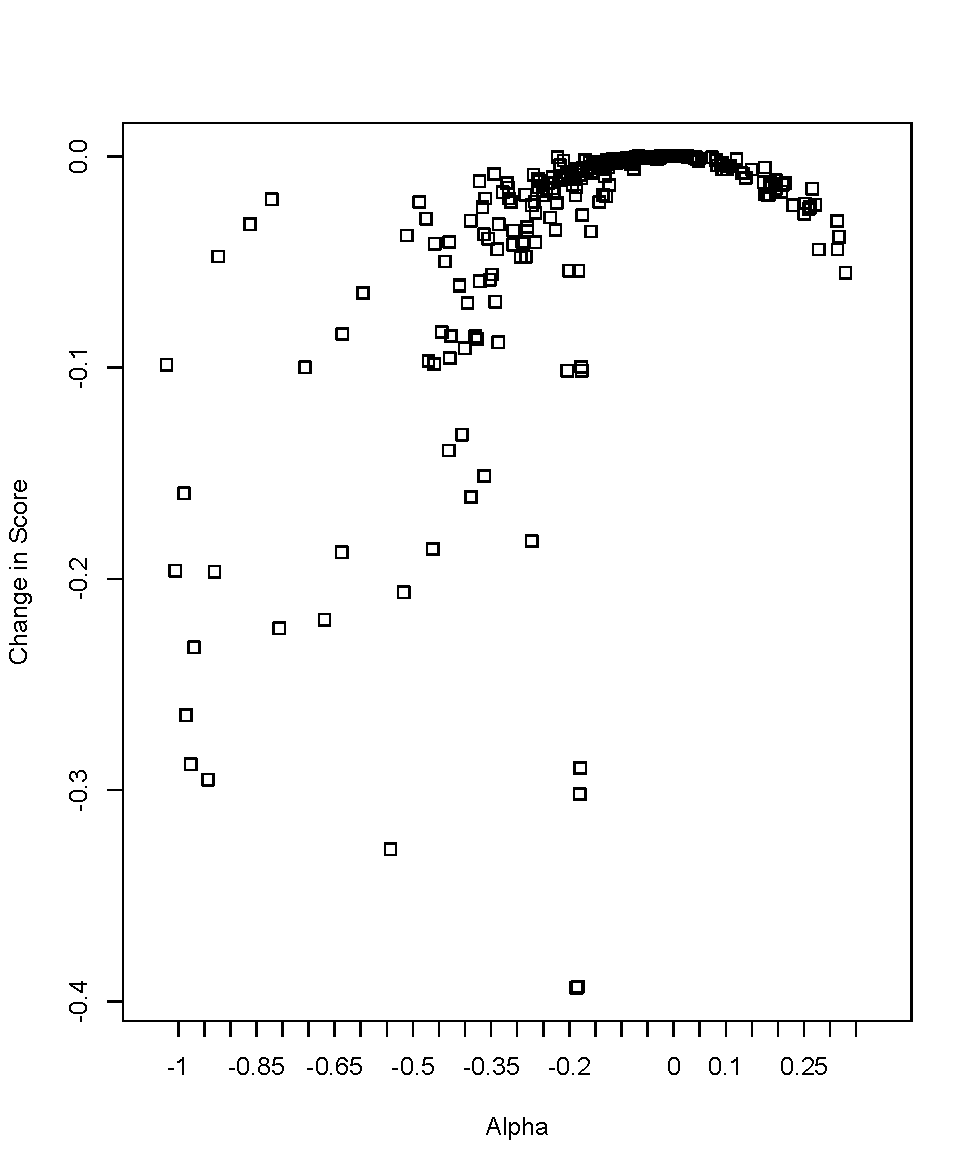
\includegraphics[width=\textwidth]{AlphaPlot.pdf}
	\caption{Kaggle team score improvements as a function of the $\alpha$ that would have maximized the scores.}
	\label{fig:alphas}
\end{figure}

The introduction of the parameter $\alpha$ to stretch or contract the estimated probabilities highlights the possibility that submitting values not equal to the actual probability estimates may be beneficial in some circumstances. To explore further, a Kaggle competitor may decide to specify a threshold, beyond which probabilities much larger (or smaller) than $0.5$ are pushed to $1$ (or $0$).
%%%%%%%%%%%%%%%%%%%%%%%%%%%%%%%%%%%%%%%%%%%
\section{Modeling}
This section details common prediction methods and then highlights our novel methodology that captures matchup specific factors. As a means for motivation, consider claims of the type ``\emph{team i is a tough matchup for team j due to their ...}'' often made by sports broadcasters. There are two ways to consider this statement: (i) the overall team strength of team $i$ will be problematic for team $j$ or (ii) team $i$ has certain tendencies above and beyond their team strength that will pose difficulties for team $j$. We outline a general framework for the first case, specifying models that account for differences in team strength. However, for the second case a different approach is needed to analytically quantify characteristics that pose difficulties for a given team. Many traditional methods, particularly those based on rankings, impose a characteristic we deem transitivity on predictions. While transitivity is fully defined in coming sections, the key point is that models with this property rely on estimates of team strength and are unable to adapt and compute specific tendencies of a given matchup. Hence, we introduce the nearest-neighbor matchup effect which captures characteristics of specific matchups and does not adhere to transitivity in predictions.  

\subsection{Data Treatment}
For our purposes game summary data is used, but another approach not explored here focuses on simulating each sequence in a game as in \cite{vstrumbelj2012} rather than the final outcome. There are a few necessary data considerations when modeling game outcomes, specifically whether the outcome of a game is binary (win/loss) or continuous (point differential) as well as whether linear or non-linear modeling (in the predictors) should be used. For the first dilemma involving whether the outcome should be modeled in a binary or continuous sense, point spread provides a means for eliciting the relative strength of one team. Although as any basketball fan can attest to the final score is often not indicative of the closeness of the game. This can go either way as fouling in the final minutes leads to inflated point differentials and often with a big lead a team will clear the bench and put in the reserves allowing the trailing team to reduce the point differential at the end of the game. Nevertheless, point spreads are informative about the relative strength of one team compared to another. In practice, given a posterior distribution of point spreads, the transformation to win probability is straightforward.  In regards to the second consideration, our experience showed that non-linear methods such as Classification And Regression Trees (CART) provided little extra predictive power when compared to linear methods. This is particularly the case when using a selection of rating systems.

\subsection{Relative Strength Models}
Adopting the continuous treatment of game outcomes, point spread, we next detail models designed to capture the relative strength of two teams. The general form for the relative strength model follows:
\begin{eqnarray}
Y_{ijk} = g_1(X_{ij}) + g_2(X_i) + g_3(X_j) +  \epsilon_{ijk}
\label{eq:RS}
\end{eqnarray}
where $Y_{ijk}$ is the point differential between teams $i$ and $j$ for matchup $k$.  The covariate matrix $X_{ij} = \{x_{ij1}, ..., x_{ijp_1}\}$ corresponds to the difference in covariates for teams $i$ and $j$, where for instance $x_{ij1} =$ Sagarin rating team $i$ - Sagarin rating team $j.$  The covariate matrix $X_l = \{x_{l1}, ..., x_{lp_2}\}$ contains predictors for team $l$, and $\epsilon_{ijk} \sim N(0,\sigma^2)$ is the error for the $kth$ matchup between teams $i$ and $j$.  Often the functions, $g_1(), g_2(),$ and $g_3()$ are linear, but they need not be. A simple example, but surprisingly useful example of Equation~\ref{eq:RS} would be a simple linear model:
\begin{eqnarray}
Y_{ijk} = X_{ij}\beta + \epsilon_{ijk}.
\label{eq:RS_Linear}
\end{eqnarray}
\subsection{Calibrating Probabilities}
Given a posterior predictive distribution for point spread between teams $i$ and $j$, $Y_{ijk},$ it is a straightforward transformation to recover win probability. Consider Figure \ref{fig:winprob} which displays the distribution of point differential and corresponding win probability for a team favored to win by 5 points (e.g. $E[Y_{ijk}|X_{ij}]=5$).
\begin{figure}[h!]
\centering
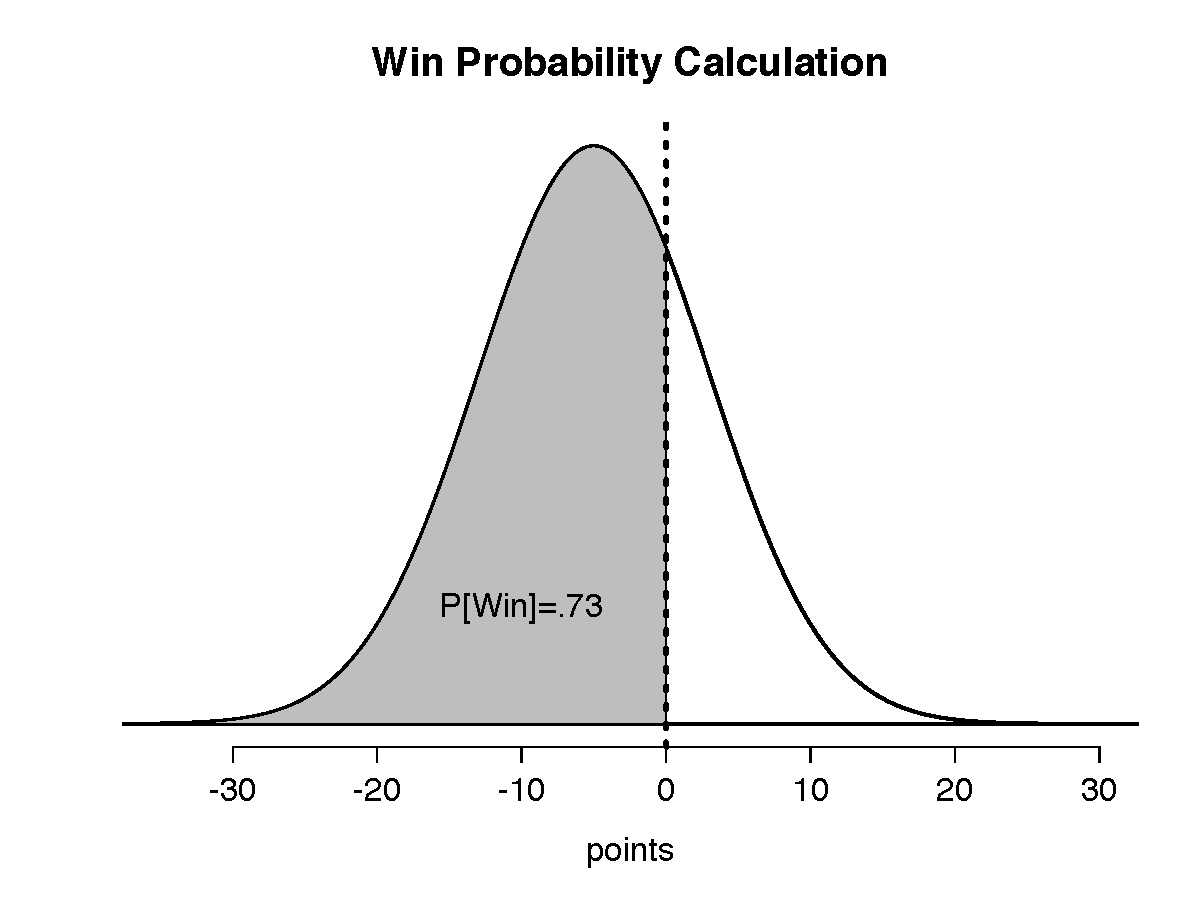
\includegraphics[width=.9\textwidth]{WinProb.pdf}
\caption{Calculating win probability from point differential}
\label{fig:winprob}
\end{figure} 
While the actual variance of the posterior predictive distribution will vary, the distribution displayed in Figure \ref{fig:winprob} is $Normal(5,11^2).$

\subsection{Popular Methods}  This section provides a review of several existing methods for tournament prediction.
\subsubsection{Rating Based Methods} 
The seeds and ratings discussed earlier contain implicit or explicit means for tournament prediction. For instance the Sagarin rankings are designed to reflect the point spread between two teams, incorporating a term for the variance of the outcomes under a Bayesian framework provides an efficient way to compute win probabilities. Similarly for any of the other rankings, coefficients for predicting point spreads or in a binary regression can be computed. A seed based probability is shown in \cite{schwertman1996}. A more sophisticated approach using point spreads along with Sagarin rankings is employed in \cite{carlin1996}. A method that allows team strength to vary in shown in \cite{glickman1998}.
\subsubsection{Ensemble Methods}
Combining the ratings from several different sites is a popular strategy. In fact this is the technique used by Nate Silver's 538 methodology. In particular Nate Silver's model incorporates 7 sets of rankings: Sagarin's, Pomeroy's, LRMC, Sonny Moore power ratings, ESPN's Basketball Power Index (BPI), NCAA selection committee ``S-curve'', and Associated Press preseason poll along with injuries and distance required to travel to construct power ratings (\cite{silver}). Similar to Sagarin's ratings, the rating difference between two teams are designed to reflect an estimated point spread. In general model averaging proved useful, smoothing out over fitting or model biases.  \cite{silver} goes on to say:
\begin{quote}
One of the ways I was able to look smart over the past six years, during which time I spent a lot of effort on political forecasting, was by betting on the favorite. I wasn't literally placing bets, mind you (unless you want to count my proposed bet with Joe Scarborough). But for some reason, in political prognostication, you can be regarded as a savant just by pointing out that the favorite is probably going to win.

The standard in sports prediction is higher. And this year's NCAA basketball tournament is designed to make me look dumb. There aren't any favorites. Sure, some teams are better bets than others. (I wouldn't advise staking your fortune on Cal Poly.) But the team that our statistical model regards as the favorite to win it all, Louisville (more on the Cardinals in a moment), has just a 15 percent chance of doing so. In other words, there�s an 85 percent chance that Louisville won't cut down the nets again and that I'll be wrong.
\end{quote}
\andyc{Consider sliding this up to intro along with Pomeroy quote}
\lucasc{@ andy, I concur, this would make a great segue into the section or the paper overall. }
\subsection{Nearest-Neighbor Matchup Effects}
The nearest-neighbor matchup effects are tailored for the second scenario in which there exist team level characteristics, above and beyond team strength, that contribute to win probability. For instance, maybe a certain team struggles with taller teams that rebound well. When facing an opponent with these attributes the team would expect to perform worse than the difference in team strengths would suggest. This is plausible as the team strength is calculated across a variety of opponents, hence we search for a subclass of opponents in which the strengths differ from the overall mean. Our procedure is a three step process: (i) fit a relative strength model of the form specified in Equation~\ref{eq:RS}, (ii) identify neighbors, by finding similarities between the current opponent and past opponents for each team, and (iii) calibrate the matchup adjustment. Fitting of the relative strength model follows the same form as previously described and will not be rehashed in this segment. Our example model which is fully detailed in the following following section follows the form of Equation \ref{eq:RS_Linear} using the Sagarin ratings as predictors.
\subsubsection{Choosing Neighbors}
When choosing neighbors for a matchup between team $i$ and team $j$, we need to identify past opponents of team $i$ with similar attributes to team $j$ and past opponents of team $j$ with similar attributes to team $i.$ The idea is to identify how the performance changes against that subset of opponents relative to the overall relative strength computed on the entire set of opponents a team has faced.

There are a multitude of ways to select the neighbors. In particular one needs to consider what variables to include for selecting neighbors, how should those variables be weighted if at all, and how many neighbors should be selected. We consider a large set of team level data from which a 5-nearest neighbor approach is calculated. In particular we use over twenty variables equally weighted for the nearest neighbor calculation including: team height, adjust tempo, percentage of scoring from 3 pointers, offensive rebound percentage, free throw percentage, block percentage, steal rate, and many others.

Typically this procedure would be done analytically, however, user input can also be solicited. For instance, suppose that a user decided Mercer was similar to Wake Forest and Clemson. In this case current and ongoing work in Bayesian Visual Analytics (BAVA) framework detailed in \cite{house2010}  and \cite{hu2013} provides a principled routine for visualizing teams and taking user input of similarities to create a method for computing distance between teams. Specifically BAVA is a way to weight clustering variables to reflect user preferences.
\subsubsection{Matchup Adjustment}
The idea of the matchup adjustment is to quantify how much a team underperformed (or over performed) relative the expected team strength for a subset of teams similar to the current opponent. For instance, if team $i$ was two points better than expected against teams similar to $j$, then it would be reasonable to assume that team $i$ would perform better against team $j$ as well.  Assume a simple linear model from Equation \ref{eq:RS_Linear}, then the predictive distribution for a matchup between team $i$ and team $j$ now becomes 
\begin{eqnarray}
p(Y_{ij}|X_{ij}, \beta,\sigma^2,\mathcal{N}_i(j),\mathcal{N}_j(i), \rho) &\sim& N(\epsilon_{ij}, \sigma^2) \label{eq:ME}
\\
\epsilon_{ij} &=& X_{ij} \beta + \rho(\mathcal{N}_i(j) -\mathcal{N}_j(i)),
\end{eqnarray}
where $\mathcal{N}_j(i) = \sum_j Y_{ijk} - E[Y_{ijk}|X_{ij}],$ is the average residual for the team $i's$ past opponents most similar to team $j$ and $\rho$ is a tuning parameter $\in [0,1]$ that controls the amount of information passed from similar neighbors. The same idea applies to the more general model specified in Equation \ref{eq:RS}.

\subsubsection{Calibrating the Matchup Adjustment}
The natural support of $\rho$ would be between zero and one.  The interpretation of the extreme points is rather intuitive - with $\rho = 0$ Equation~\ref{eq:ME} reverts to Equation~\ref{eq:RS} and with $\rho = 1$ the entire residual for similar teams is retained. To select $\rho$ in practice, we recommend a historical analysis to calibrate $\rho$ for the current year's predictions. For the relative strength model and nearest neighbor variables used in this work, $\rho$ near 0.2 performed optimally across the historical data.   \andyc{maybe add the plot Marcos suggested here showing historical effect of $\rho$??}.

\subsection{A note about Transitivity}
The transitive property states if $A>B$ and $B>C$ then $A>C$. In terms of basketball prediction consider:
\begin{eqnarray}
P_{A,B} > 0.5 \quad \& \quad P_{B,C} > 0.5 \rightarrow P_{A,C} > 0.5,
\label{eq:trans}
\end{eqnarray}
where $P_{I,J}$ is the probability of team I defeating team J.  We deem Equation \ref{eq:trans} a transitive property for basketball prediction. This means if team A is expected to beat team B and team B is expected to beat team C, then team A should also defeat team C. Note these are probabilities not true outcomes, due to the parity in basketball inferior teams can and often do defeat stronger teams. Any sort of relative strength model would require this transitive ordering holds, home court effects non-withstanding. On the other hand, our matchup effects modeling approach can determine if the strengths of a given team present difficulties for a specific team meaning the transitive property is not required to hold and $P_{A,B} > 0.5 \quad \& \quad P_{B,C} > 0.5\quad \& \quad P_{A,C} < 0.5$ is valid.
%%%%%%%%%%%%%%%%%%%%%%%%%%%%%%%%%%%%%%%%%%%
\section{Evaluation}
The evaluation section contains three distinct components: an analysis of the performance of a few popular methods, an overview of the Kaggle predictions, and a demonstration of the Nearest Neighbor Matchup Effects.
\subsection{Popular Methods}
March Madness prediction draws the attention of sport analysts and medias: notably, Nate Silver, Ken Pomeroy and the ESPN. In this section, we will compare these three models against Kaggle entries and examine the ``luck'' factor of Kaggle competition.

Because Silver and Pomeroy published probabilities of each team advancing, our first comparison focused on first round games (round of 64).  We noticed that all three models concurred in win-loss predictions except for one game (Gonzaga vs OKST, 8 vs 9 in West). All three models have a similar pattern based on the predictions' deviation from 0.5: while most predictions either suggest a easy win (prediction close to 1) or a close game (prediction close to 0.5), predictions around 0.75 are relatively rare in all three models.

In addition, Silver's prediction adopted a more aggressive style than the other two. His prediction, on average, has the highest deviation from 50-50 prediction and Pomeroy has the lowest. But this difference seems to be irrelevant to their scores. For the first around games, Pomeroy has the best score at 0.4632, followed by Silver 0.4664 and ESPN 0.4709. These scores ranked 38th, 45th and 64th respectively, among 433 Kaggle entries. 

We also computed a full-scale, team-to-team prediction based on the marginal advancement probabilities and found both the score and ranking of three models have dropped markedly from first round: ESPN (0.5795, 88th), Silver(0.5988, 123rd) and Pomeroy (0.6278, 174th). 

Another interesting finding in this comparison is the ``luck'' factor. What if a close game finished differently? To that end, we flipped the five overtime games in the first round and noticed a completely reverse of the ranking of popular models: ESPN(0.4631, 11th), Silver(0.5025,117th) and Pomeroy (0.5027,120th). This phenomenon is observed in other Kaggle entries as well. A 0.7169 Kendall's Tau is measured between the rankings before and after flipping. 

To sum up, popular models exhibit similarities in many aspects,  but none has shown clear advantages over most Kaggle entries. 

\subsection{Kaggle Leaderboard}
\andyc{is this section appropriate here?  Consider the flow of the paper once  the pieces come together}
\subsection{Nearest Neighbor Matchup Effects}
To demonstrate the efficacy of our method, we first fit Equation~\ref{eq:RS} using a well known rating system, the Sagarin ratings. After fitting this model, $\rho$ is calibrated based on historical results from the previous seven years NCAA tournaments. Seven years was chosen because this is the length of the complete history of the team level characteristics used to find neighbors of teams. The log loss for 2014 for the entire range of $\rho$ can be seen in Figure~\ref{fig:result} and in particular the reduced loss for the $\rho=0.2$ that was selected based on historical calibration.
\begin{figure}[h!]
\centering
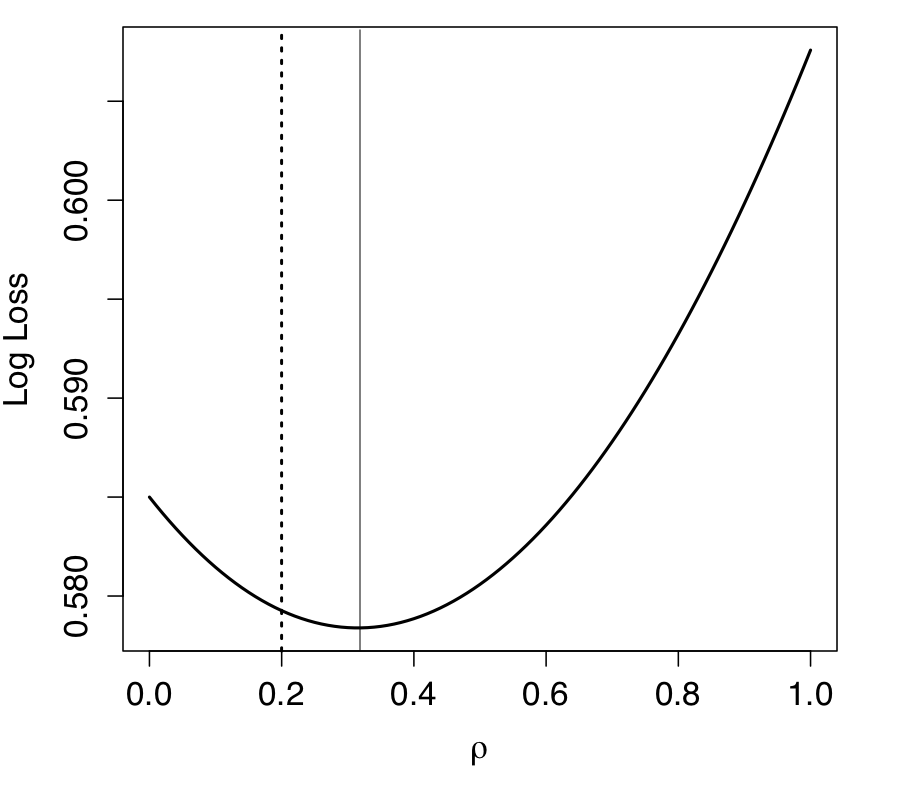
\includegraphics[width=.7\textwidth]{results_2014.pdf}
\caption{Solid Line: Log loss for $\rho$, dashed vertical line: $\rho=.2$ value selected by historical calibration}
\label{fig:result}
\end{figure} 
A modest improvement is also seen in classification error from (0.365 to 0.350) although this is only a single game difference. The matchup effect, particularly with smaller $\rho$ values, will have a lesser effect on classification error than that of the loss functions like the log loss. This is because it will only shift the expected point differential a small margin, so the only games in which classification error would change are those that are nearly dead heat games to begin with.

To illustrate the matchup effects, consider Table~\ref{tab:change} which contains the ten games that saw the largest shift in expected point differential. This table contains expected point differentials (team1 - team2) denoted as Point Diff for the relative strength model (RS) as well as the matchup effects (ME).  Similarly probabilities of team 1 winning and realized loss for each model are depicted.  Finally the actual point differential is shown.
\begin{table}[h!]
\caption{ Ten games with largest point differential change when implementing Nearest Neighbor Matchup Effects model versus a relative strength model}
\scriptsize
\centering
\begin{tabular}{|cc | ccc | ccc | c|c|}
  \hline
  \hline
 team 1 & team 2 & Point Diff:RS & Prob:RS & Loss:RS & Point Diff:ME & Prob:ME & Loss:ME & Point Diff\\ 
  \hline
 Cal Poly & Wichita St & -18.69 & 0.04 & 0.04 & -17.10 & 0.06 & 0.06 &  -27\\ 
 UConn & St. Joes &4.29 & 0.65 & 0.43 & 6.18 & 0.71 & 0.34 & 8\\ 
 Dayton & Stanford & -2.16 & 0.42 & 0.86 & 0.94 & 0.53 & 0.63 & 10 \\ 
 Dayton & Syracuse & -6.34 & 0.28 & 1.27 & -4.05 & 0.36 & 1.03 & 2\\ 
 Kentucky & Michigan & -3.71 & 0.37 & 1.00 & -2.08 & 0.42 & 0.86 &  3\\ 
 UMass & Tennessee &-3.05 & 0.39 & 0.49 & -4.83 & 0.33 & 0.40 & -19\\ 
 Memphis & Virginia & -6.34 & 0.28 & 0.33 & -8.91 & 0.21 & 0.23 & -18\\ 
 Michigan & Tennessee & 5.37 & 0.69 & 0.37 & 3.49 & 0.62 & 0.47 & 2\\ 
 Michigan & Texas & 8.05 & 0.77 & 0.26 & 5.85 & 0.70 & 0.35 & 14\\ 
 Syracuse & W. Mich. & 12.65 & 0.88 & 0.13 & 15.01 & 0.92 & 0.09 & 24\\ 
   \hline
   \hline
\end{tabular}
\label{tab:change}
\end{table}
The key takeaway from this table is the loss for the predictions under each methodology. On this particular subset of games, the ME model performs considerably better than the typical model under the log loss (.446 to .520), the other games see minimal matchup effects, therefore, the results are similar.  To further illustrate how the nearest neighbor match effects functions consider the Dayton versus Stanford game.  Coincidentally this is the only game which the actual predicted winner changes, while many saw sizable shifts in predictive probabilities which factor into the loss function used in the Kaggle competition.  For each team, Table \ref{tab:DayStan} displays the neighbors, that is opponents that they faced most similar to the current matchup, along with the expected differential, realized result, and residual in those games. 
\begin{table}[h!]
\caption{Dayton - Stanford Neigbors \& Residuals}
\small
\centering
\begin{tabular}{|c|cccc |}
   \hline
   \hline
 team & neighbor &  Point Diff& Exp. Point Diff & Residual \\
  \hline
Dayton & California & 18 & -0.9 & 18.9\\
Dayton & Gonzaga & 5 & -12.4 & 17.4\\
Dayton & George Mason& 17 & 3.4 & 13.6\\
Dayton &  Georgia Tech& 10 & -5.3 & 15.3\\
Dayton & George Washington& 10 & 0.4 & 9.6\\
\hline
Stanford & California&-7 & 4.1&-11.1 \\
Stanford & California &11 &-2.3 &13.3 \\
Stanford & Oregon&2 &-8.9 &10.9 \\
Stanford & Pittsburgh&-21 &-5.3 &-15.7 \\
Stanford & Cal Poly&17 &13.8 &3.2 \\
Stanford & Utah&1 &4.9 &-3.9 \\
   \hline
   \hline
\end{tabular}
\label{tab:DayStan}
\end{table}
To avoid confusion one of Stanford's five neighbors was the University of California at Berkeley, who they faced twice.  The difference in expected point differential is driven largely by the fact that the first game was at Stanford while the second was at Berkeley. From this table we see that Dayton performed exceptionally well against teams our model considered to be similar to Stanford, in fact they were about 15 points better on average. The line shifted more than 3 points for this game because $\rho$ was calibrated to 0.2.
%%%%%%%%%%%%%%%%%%%%%%%%%%%%%%%%%%%%%%%%%%%

\section{Luck}
\lucasc{@Ian, this is something from the forum on the kaggle comp, it is answering a question about scoring predictions. }
\ianc{What's this guy talking about?}
\noindent It's not about the prize, it's the element of luck involved...\\
\noindent  William Cukierski, Kaggle Competition Admin \\

Previously, we detailed popular methods for prediction and outlined our new methodology that accounts for specific match ups. In this section of this paper, we address the high degree of chance present in NCAA tournaments and consequently prediction for NCAA tournaments.  Specifically, we address sensitivity of a Kaggle style leader board. While it is natural to think 2nd place almost won, we aim to answer the question how close was 20th place to winning? 

% some verbiage in here... 

To study the effect of luck we take the idea that the 2nd place team almost won and we attempt to quantify `almost.' To this end, we examine alternate realities where a losing team in an overtime game is treated instead as a winning team. We focus only on overtime games because it seems most reasonable to think of the losing team as having won in those cases. Recall that the loss function used for scoring of the Kaggle competition is

\lucasc{Maybe we can omit this equation if it is defined in an earlier section and just number that version and refer to that equation number here?} 
\begin{equation}\label{eqn:kaggle_score}
-\sum_{i=1}^n\frac{y_ilog(p_i)+ (1-y_i)log(1-p_i)}{n},
\end{equation}
where $y_i$ is a binary variable taking value 1 when the team wins and 0 otherwise and $0 \leq p_i \leq 1$ denotes the predicted value for the team in the $i$th game. We consider how dependent the rankings of individual teams are on the characteristics of the particular loss function. To answer this question we studied a couple of possible alternate scoring functions. We consider the following scoring functions: 
 
\begin{equation}\label{eqn:first_score_function}
-log(1-2|.5-p_i|)
\end{equation} 

\begin{equation}\label{eqn:second_score_function}
-log(1-|.5-p_i|)
\end{equation} 

\begin{equation}\label{eqn:third_score_function}
-log(1-|y_i-p_i|)
\end{equation} 
Here, for brevity, we only write the part of the loss function multiplied by the $(1-y_i)$ term. Moreover, in Function \ref{eqn:third_score_function}, $y_i \in \{0,.5,1\}$, where now the $0.5$ is the realized value when teams go into overtime, the other equations use only $y_i \in \{0,1\}$. Figure \ref{fig:scoring_functions} is a plot of the different score functions for values $0\leq p_i \leq 1$.  

\ianc{It's not clear how these functions correspond to the lines in the plot below. We're also not sure that it's necessary to consider so many marginally different loss functions.}

\begin{figure}[H]
\centering
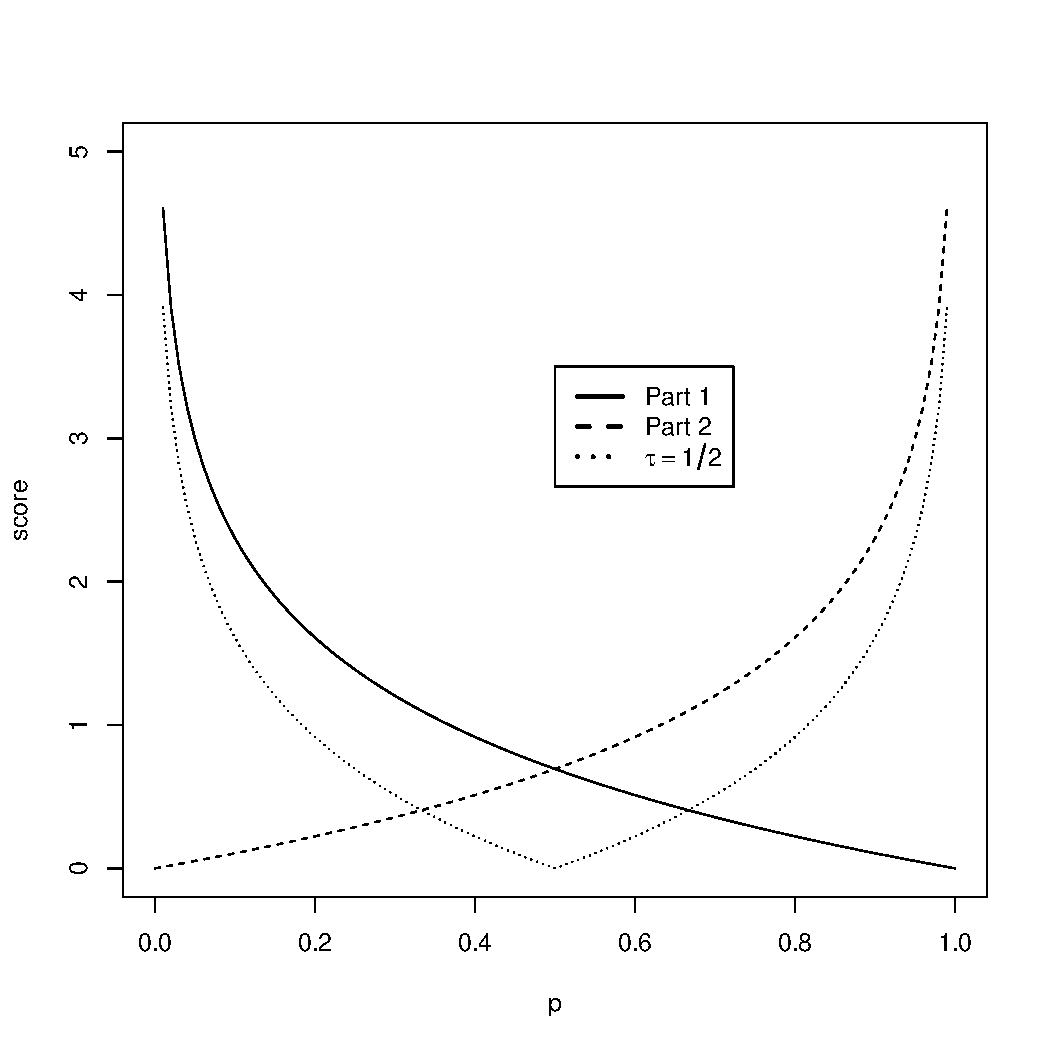
\includegraphics[width=.7\textwidth]{loss_function_plot_bw.pdf}
\caption{A plot of the various loss functions as a function of the prediction $p_i$.  }
\label{fig:scoring_functions}
\end{figure}

It is clear from looking at Figure \ref{fig:scoring_functions} that the different scoring functions treat the contestant's confidence differently. Both Equations \ref{eqn:first_score_function} and \ref{eqn:second_score_function} are symmetric about 0.5, which is aesthetically pleasing and a useful attribute for handling tied or overtime games in a slightly different manner than games with a clear victor. Moreover, Equation \ref{eqn:first_score_function} penalizes much more for confident predictions than Equation \ref{eqn:second_score_function}. 

One might wonder, given the plethora of choices one might use to rank contestants, how much is a result of a specific scoring function and how much much change of  we moved from one scoring function to another? To examine this, we made a plot of the contestant predictions scored under the various loss functions described above. The results of this plot are shown in Figure \ref{fig:score_rank_plot}. 

  \begin{figure}[h]
\centering
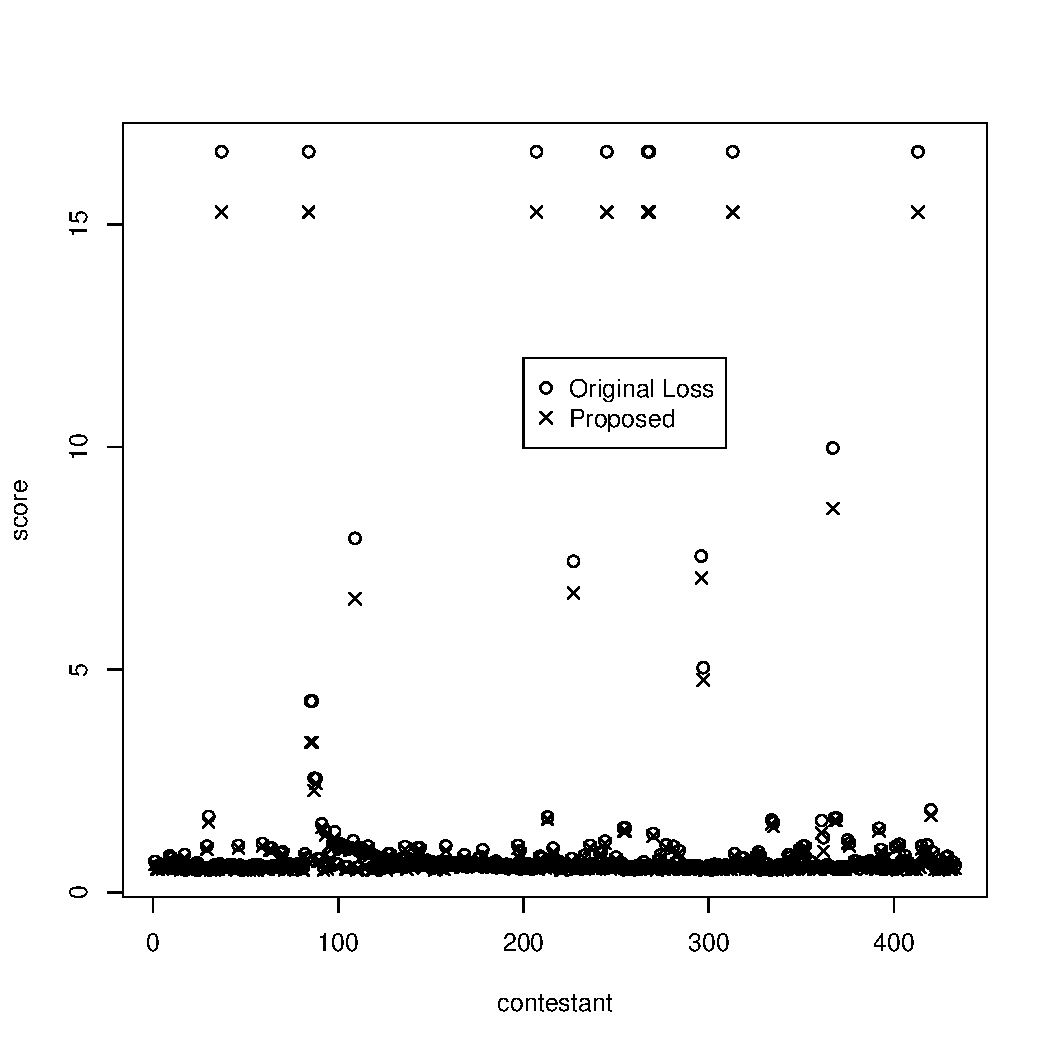
\includegraphics[width=.7\textwidth]{prelim_rank_plot1_bw.pdf}
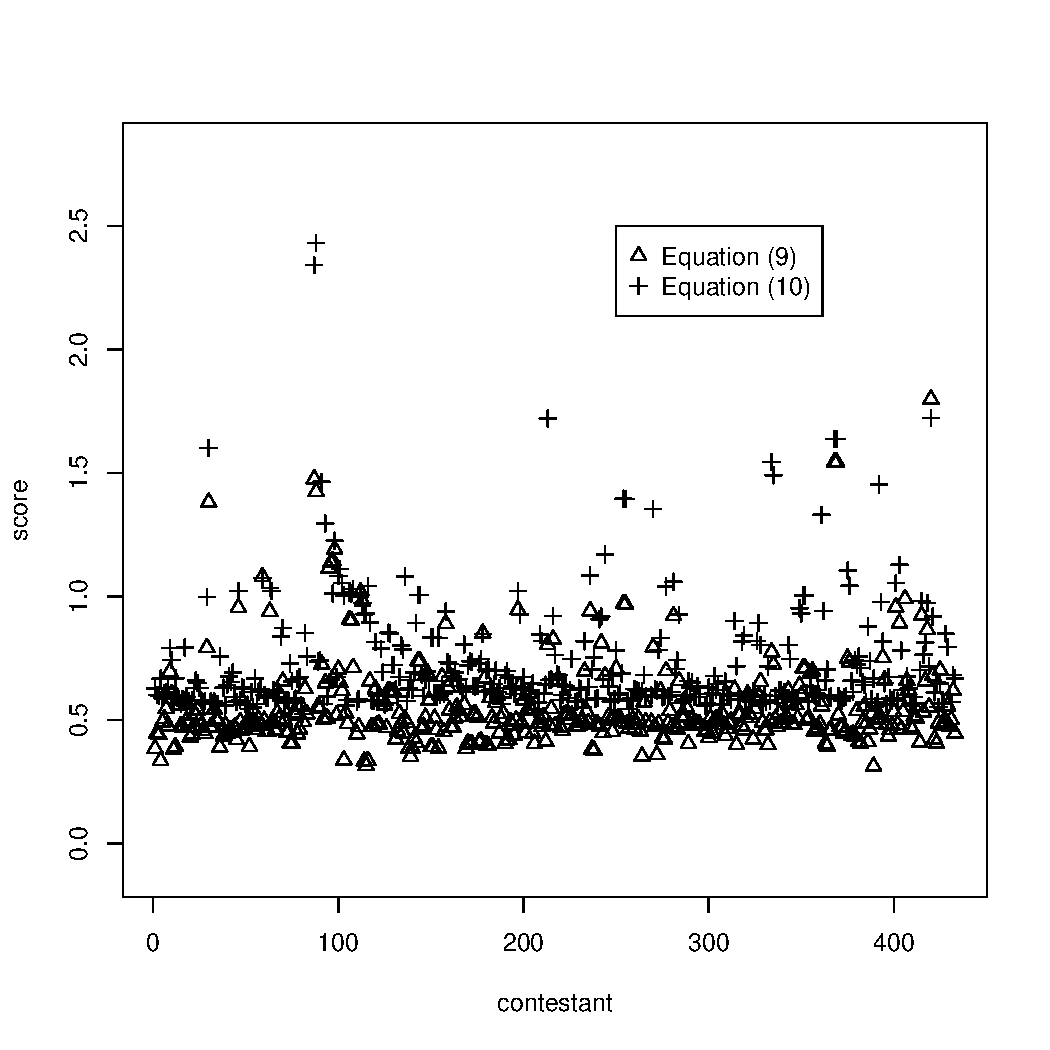
\includegraphics[width=.7\textwidth]{prelim_rank_plot2_bw.pdf}

\caption{The scores of each contestant under the different loss functions. A smaller score is better.  }
\label{fig:score_rank_plot}
\end{figure}

Given that the choice of scoring function can affect the contestants' positions on the leaderboard, we did a correlation analysis of the contestant submissions resulting from the actual scoring function, Equation \ref{eqn:kaggle_score} and correlated these ranks against the ranks of the contestants under the other three scoring functions. The results of this analysis are shown in Table \ref{tab:kendall_tau_table} beneath. There appear to be little correlation between the resultant rankings, indeed, there was not a single significant p-value amongst the results.  Of course one might think, there can be little overall correlation between the rankings but still the top three might be the same or similar across the various scoring functions but this turned out not to be the case. In fact, comparing the top three on the leaderboards for the different scoring functions show no common contestants. Additionally, we looked at the three worst contestants as well, here the trend was the same, no common contestants when scoring using different criteria. 

\begin{table}[ht]
\centering
\begin{tabular}{rrr}
  \hline
Score comparison & $\tau$ & p-value \\ 
  \hline
\ref{eqn:kaggle_score} vs. \ref{eqn:first_score_function} & -0.00 & 0.97 \\ 
\ref{eqn:kaggle_score} vs. \ref{eqn:second_score_function} & 0.01 & 0.79 \\ 
\ref{eqn:kaggle_score} vs. \ref{eqn:third_score_function} & 0.05 & 0.09 \\ 
\ref{eqn:first_score_function} vs. \ref{eqn:second_score_function} & -0.03 & 0.42 \\ 
\ref{eqn:first_score_function} vs. \ref{eqn:third_score_function}   & -0.05 & 0.15 \\ 
\ref{eqn:second_score_function} vs. \ref{eqn:third_score_function}  & 0.00 & 0.96 \\ 
   \hline
\end{tabular}
\label{tab:kendall_tau_table}
\caption{}
\end{table}



Leakage is defined by \cite{schutt2013doing} as an accidental inclusion of `future' data into the training set. \cite{schutt2013doing} state that in earlier days of online comptitions they were able to consistently win competitions by systematically exploiting leakage. While much has been made in contest forums and in books  about leakage and how leakage is often exploited to win competitions, it is somewhat refreshing to see that other choices like the scoring function play into the relative results of a competition. While leakage might be the result of competition administrators' errors, or a misunderstanding of the data generating process, the scoring function should be chosen to match the reality of the errors made while forecasting. While luck ultimately plays a role in the basketball games themselves and the results of prediction tournaments, some players are able to consistently outperform. While this section has depicted alternate outcomes that could have occurred, an actual alternate outcome will not arise until next year when the tournament occurs.  These consistent outperformers are lucky, but lucky in the sense that they managed to get the right results for their specific loss function used in the competition. The results shown here indicate that if a contestant does not explicitly incorporate the loss function into their predictions, they are leaving their winnings more to chance than to skill. 
%%%%%%%%%%%%%%%%%%%%%%%%%%%%%%%%%%%%%%%%%%%
\section{Recommendations}
In general NCAA bracket competitions, \cite{niemi2008} and \cite{breiter1997} provide a good overview of optimal strategies.  As probabilistic predictions are a bit different we highlight some high level ideas and then provide more detailed recommendations. Our takeaway from this competition is that high quality data, reasonable models, and a little luck are the components for a successful modeling competition. This is echoed by \cite{kaggle}, the winning Kaggle competitors.
\begin{quote}
Q: Were you surprised by any of your insights?

Greg: I was surprised by how well our simple models performed. Using the right data was MUCH more important to our models performing well than using more sophisticated models.

Mike: I think we gave ourselves a chance with a good model, but there was probably a decent amount of luck involved, too. Also, identifying the specific loss function for this Kaggle contest, and where it comes from, seemed to help our model.
\end{quote}
We also found that there seemed to be little advantage in using complex models as simple linear models worked quite well.  Something that was beneficial was modeling point spread rather than treating wins and losses in a binary sense, this agrees with  \cite{gelman}:
\begin{quote}
Don't model the probability of win, model the expected score differential. Yeah, I know, I know, what you really want to know is who wins. But the most efficient way to get there is to model the score differential and then map that back to win probabilities. The exact same issue comes up in election modeling: it makes sense to predict vote differential and then map that to Pr(win), rather than predicting Pr(win) directly. This is most obvious in very close games (or elections) or blowouts; in either of these settings the win/loss outcome provides essentially zero information. But it's true more generally that there's a lot of information in the score (or vote) differential that�s thrown away if you just look at win/loss.
\end{quote}
Next we provide more detailed strategies for probabilistic modeling competitions.
\subsection{Optimal Strategies}
\andyc{Marcos's piece here}
How should a typical user use this to figure out their bracket/Kaggle competition?
%%%%%%%%%%%%%%%%%%%%%%%%%%%%%%%%%%%%%%%%%%%
\section{Discussion}
As shown in the the section on luck, chance coupled with a relatively small sample size makes winning NCAA prediction competitions a difficult task.  Nevertheless, we provide some sound methods and techniques for making game-by-game predictions. Our matchup effects model is an intuitive means for adjusting probabilities based on matchup specific characteristics. While there undoubtably is a more principled way to carry out this exercise, and given the time constraints, we found this to be effective.

Other considerations would be to use injury data for players as Nate Silver's 538.com does. However, this particular competition required predictions for the complete tournament in advance of the first games. Nevertheless, knowing the status of Kansas's Joel Embiid would have shifted probabilities for Kansas and similarly the effect of Iowa State's Georges Niang injury prior to the sweet sixteen matchup with Connecticut would undoubtedly have lead to different predictive values

Something else that may be beneficial would be to use the score with two minutes to go, for example, to quantify how a game was. As any fan can attest, the strategy of fouling can lead to dramatically different scores as can garbage time minutes by reserves, which results in a distorted view of how close the game was. However, the time constraints for this year's competition deterred us from pursuing this - perhaps next year.

%%%%%%%%%%%%%%%%%%%%%%%%%%%%%%%%%%%%%%%%%%%
%%%%%%%%%%%%%%%%%%%%%%%%%%%%%%%%%%%%%%%%%%%

\bibliographystyle{DeGruyter}
\bibliography{refsJQAS}

%%%%%%%%%%%%%%%%%%%%%%%%%%%%%%%%%%%%%%%%%%%
%%%%%%%%%%%%%%%%%%%%%%%%%%%%%%%%%%%%%%%%%%%

%%%%%%%%%%%%%%%%%%%%%%%%%%%%%%%%%%%%%%%%%%%


%%%%%%%%%%%%%%%%%%%%%%%%%%%%%%%%%%%%%%%%%%%

\end{document}
